\chapter{Evaluation and Validation}
\label{chap:evaluation}

This chapter presents the systematic evaluation and validation of the\ac{VMAP} database system. Following the implementation described in Chapter \ref{chap:implementation}, a comprehensive testing strategy was developed to assess the system's functionality, performance, and compliance with requirements. The evaluation process focused on four key areas: user management, release management, parameter versioning, and variant management, using both controlled test scenarios and production-scale data volumes. Rather than an exhaustive documentation of all tests, this chapter highlights representative test cases and key findings that demonstrate the system's capabilities and limitations.

\section{Validation Methodology}
\label{sec:validation-methodology}

The validation methodology followed a structured approach combining functional testing, performance analysis, and integration verification. To ensure realistic evaluation, both baseline and production-scale datasets were used, with the baseline dataset containing approximately 20,000 parameters across 2 \acp{ECU}, and the production-scale dataset containing over 100,000 parameters across 5 \acp{ECU}.

\subsection{Test Scenario Development}
\label{subsec:test-scenario-development}

Test scenarios were developed based on actual automotive parameter management workflows identified during requirements analysis in Chapter \ref{chap:methodology}. Each test scenario was designed to validate specific functional requirements while reflecting real-world usage patterns. The scenarios incorporated representative tasks for each user role and followed complete workflow sequences from parameter definition through variant creation to documentation.

The test scenarios were categorized into functional areas corresponding to the primary system capabilities:

\begin{itemize}
\item \textbf{User Management}: Authentication, authorization, role assignment, module access
\item \textbf{Release Management}: Phase transitions, freeze operations, phase comparison
\item \textbf{Variant Management}: Variant creation, segment modification, inheritance
\item \textbf{Integration}: PDD synchronization, vehicle configuration
\end{itemize}

Each scenario was implemented as a structured test case with defined inputs, expected outcomes, and verification steps at both the application and database levels. The test design followed a modified version of Molinaro's approach to database validation \cite{molinaro2005sql}, with additional emphasis on traceability between requirements and test cases.

\subsection{Performance Measurement Framework}
\label{subsec:performance-measurement-framework}

A performance measurement framework was established to assess system responsiveness and resource utilization under various operational conditions. Key performance indicators were defined based on system requirements, including query response time, transaction throughput, database size growth patterns, memory utilization, and execution time for batch operations. 

Performance measurements were conducted on a standardized test environment matching the target production specifications: PostgreSQL 17 running on a server with 8 vCPUs, 32GB RAM, and SSD storage. All tests were performed with both the baseline dataset and the production-scale dataset to assess scaling characteristics.

The measurement methodology employed automated test scripts with integrated timing capture, following the principles outlined by Zaitsev et al. \cite{schwartz2012high} for database performance evaluation. Each test was executed multiple times with results averaged to account for system variations, and outliers were identified and analyzed for potential optimization opportunities.

\section{Functional Testing Results}
\label{sec:functional-testing-results}

Functional testing validated the core capabilities of the\ac{VMAP} system against the requirements defined in Chapter \ref{chap:methodology}. This section presents the key findings for each functional area, focusing on representative test cases and critical system behaviors.

\subsection{User Management Validation}
\label{subsec:user-management-validation}

The user management and access control system was evaluated to verify the implementation of the hybrid role-permission model described in Section \ref{subsec:user-role-requirements}. Testing focused on verifying that the implemented database schema and logic correctly enforced the defined access control rules for each user role. As Sandhu et al. \cite{sandhu1998role} emphasize, effective evaluation of role-based access control requires testing both positive permissions (granted access) and negative permissions (denied access) across role boundaries.

A test matrix was developed covering key permission boundaries: role-based permissions, module-based access control, direct permission assignment, and phase-specific permissions. Each test case verified a specific permission boundary with validation at both service and database layers. This focused approach aligns with Molinaro's principles for database validation \cite{molinaro2005sql}, which emphasizes targeted verification of critical constraints.

Table \ref{tab:module-dev-test-cases} presents a representative sample of test cases that focus on the Module Developer role, illustrating the connection between functional requirements and verification scenarios.

\begin{table}[H]
\centering
\caption{Sample Module Developer Role Permission Test Cases}
\label{tab:module-dev-test-cases}
\begin{tabular}{|p{0.7cm}|p{3.5cm}|p{3.7cm}|p{3.7cm}|c|}
\hline
\textbf{ID} & \textbf{Description} & \textbf{Test Action} & \textbf{Expected Outcome} & \textbf{Status} \\
\hline
MD-01 & Create Variant (Assigned Module) & Create new variant for parameter in assigned module & Variant created successfully & Pass \\
\hline
MD-02 & Create Variant (Unassigned Module) & Create new variant for parameter in unassigned module & Access denied error & Pass \\
\hline
MD-03 & Edit Variant (Assigned Module) & Modify existing variant code rule & Variant updated successfully & Pass \\
\hline
MD-04 & Delete Variant & Attempt to delete variant & Access denied error & Pass \\
\hline
MD-05 & Create Segment (Assigned Module) & Create new segment with valid value & Segment created successfully & Pass \\
\hline
MD-06 & Modify Frozen Phase & Attempt to modify segment in frozen phase & Access denied error & Pass \\
\hline
\end{tabular}
\end{table}

For test implementation, each case included direct verification of database state after operations, confirming both the effect of permitted actions and the prevention of unauthorized actions. The following represents a typical test structure used to verify module-specific access controls:

\begin{lstlisting}[language=CSharp, caption={Representative Test Case Structure}, label={lst:test-case-structure}]
// Scenario: Module Developer attempting to create variant in unassigned module
// Arrange: Set up test user and unassigned module parameter
var user = GetTestUser("module_developer@example.com");
var unassignedParameter = GetParameterFromUnassignedModule();
var variant = CreateVariantForParameter(unassignedParameter);

// Act & Assert: Verify permission is denied
var exception = Assert.Throws<PermissionDeniedException>(() => 
    _variantService.CreateVariant(variant, user.UserId));
Assert.That(exception.Message, Contains.Substring("No write access"));

// Verify no database change occurred
var dbVariant = _database.QuerySingleOrDefault<Variant>(
    "SELECT * FROM variants WHERE name = @Name", 
    new { Name = variant.Name });
Assert.IsNull(dbVariant);
\end{lstlisting}

The module-based access control tests verified that write access was correctly limited to assigned modules for Module Developers while read access remained available for all modules, implementing the principle of least privilege as recommended by Sandhu and Bhamidipati \cite{sandhu1997arbac97}. Direct permission assignment tests confirmed that user-specific permissions effectively overrode role defaults, a capability essential for supporting exception cases in complex organizational structures as noted by Hu et al. \cite{hu2015implementing}.

Phase-specific permission tests validated the interaction between the access control system and the phase management framework, confirming that modifications to frozen phases were properly prevented while still allowing appropriate access for documentation purposes. This validation addresses a critical requirement for regulated development processes as described by Staron \cite{staron2021automotive}, where development milestone integrity must be preserved.

\begin{table}[h]
    \centering
    \caption{User Management Test Results}
    \label{tab:rbac-test-results}
    \begin{tabular}{|p{3cm}|p{5cm}|}
    \hline
    \textbf{Test Category} & \textbf{Results} \\
    \hline
    Role Permission Validation & Core permissions correctly applied through roles \\
    \hline
    Module-Based Access & Write access correctly limited to assigned modules \\
    \hline
    Direct Permission Assignment & User-specific permissions overrode role defaults \\
    \hline
    Phase-Specific Permissions & Frozen phase protection enforced correctly \\
    \hline
    \end{tabular}
\end{table}

The audit trail verification confirmed that security-related operations were properly logged with complete metadata, including the user making the change, timestamp, and specific permissions affected. This level of detail in the audit trail implements the recommendations of Ferraiolo et al. \cite{ferraiolo2011policy} for maintaining accountability in security-sensitive operations.

\subsection{Module Access Impact on Performance}
\label{subsec:module-access-impact}

The impact of module-specific access checks on performance was evaluated as part of the access control testing. This analysis focused on understanding the performance overhead introduced by adding module-specific access verification to the standard permission checking process. Figure \ref{fig:module-access-impact} illustrates the measured performance difference between standard permission checks and combined permission and module access checks.

\begin{figure}[h]
    \centering
    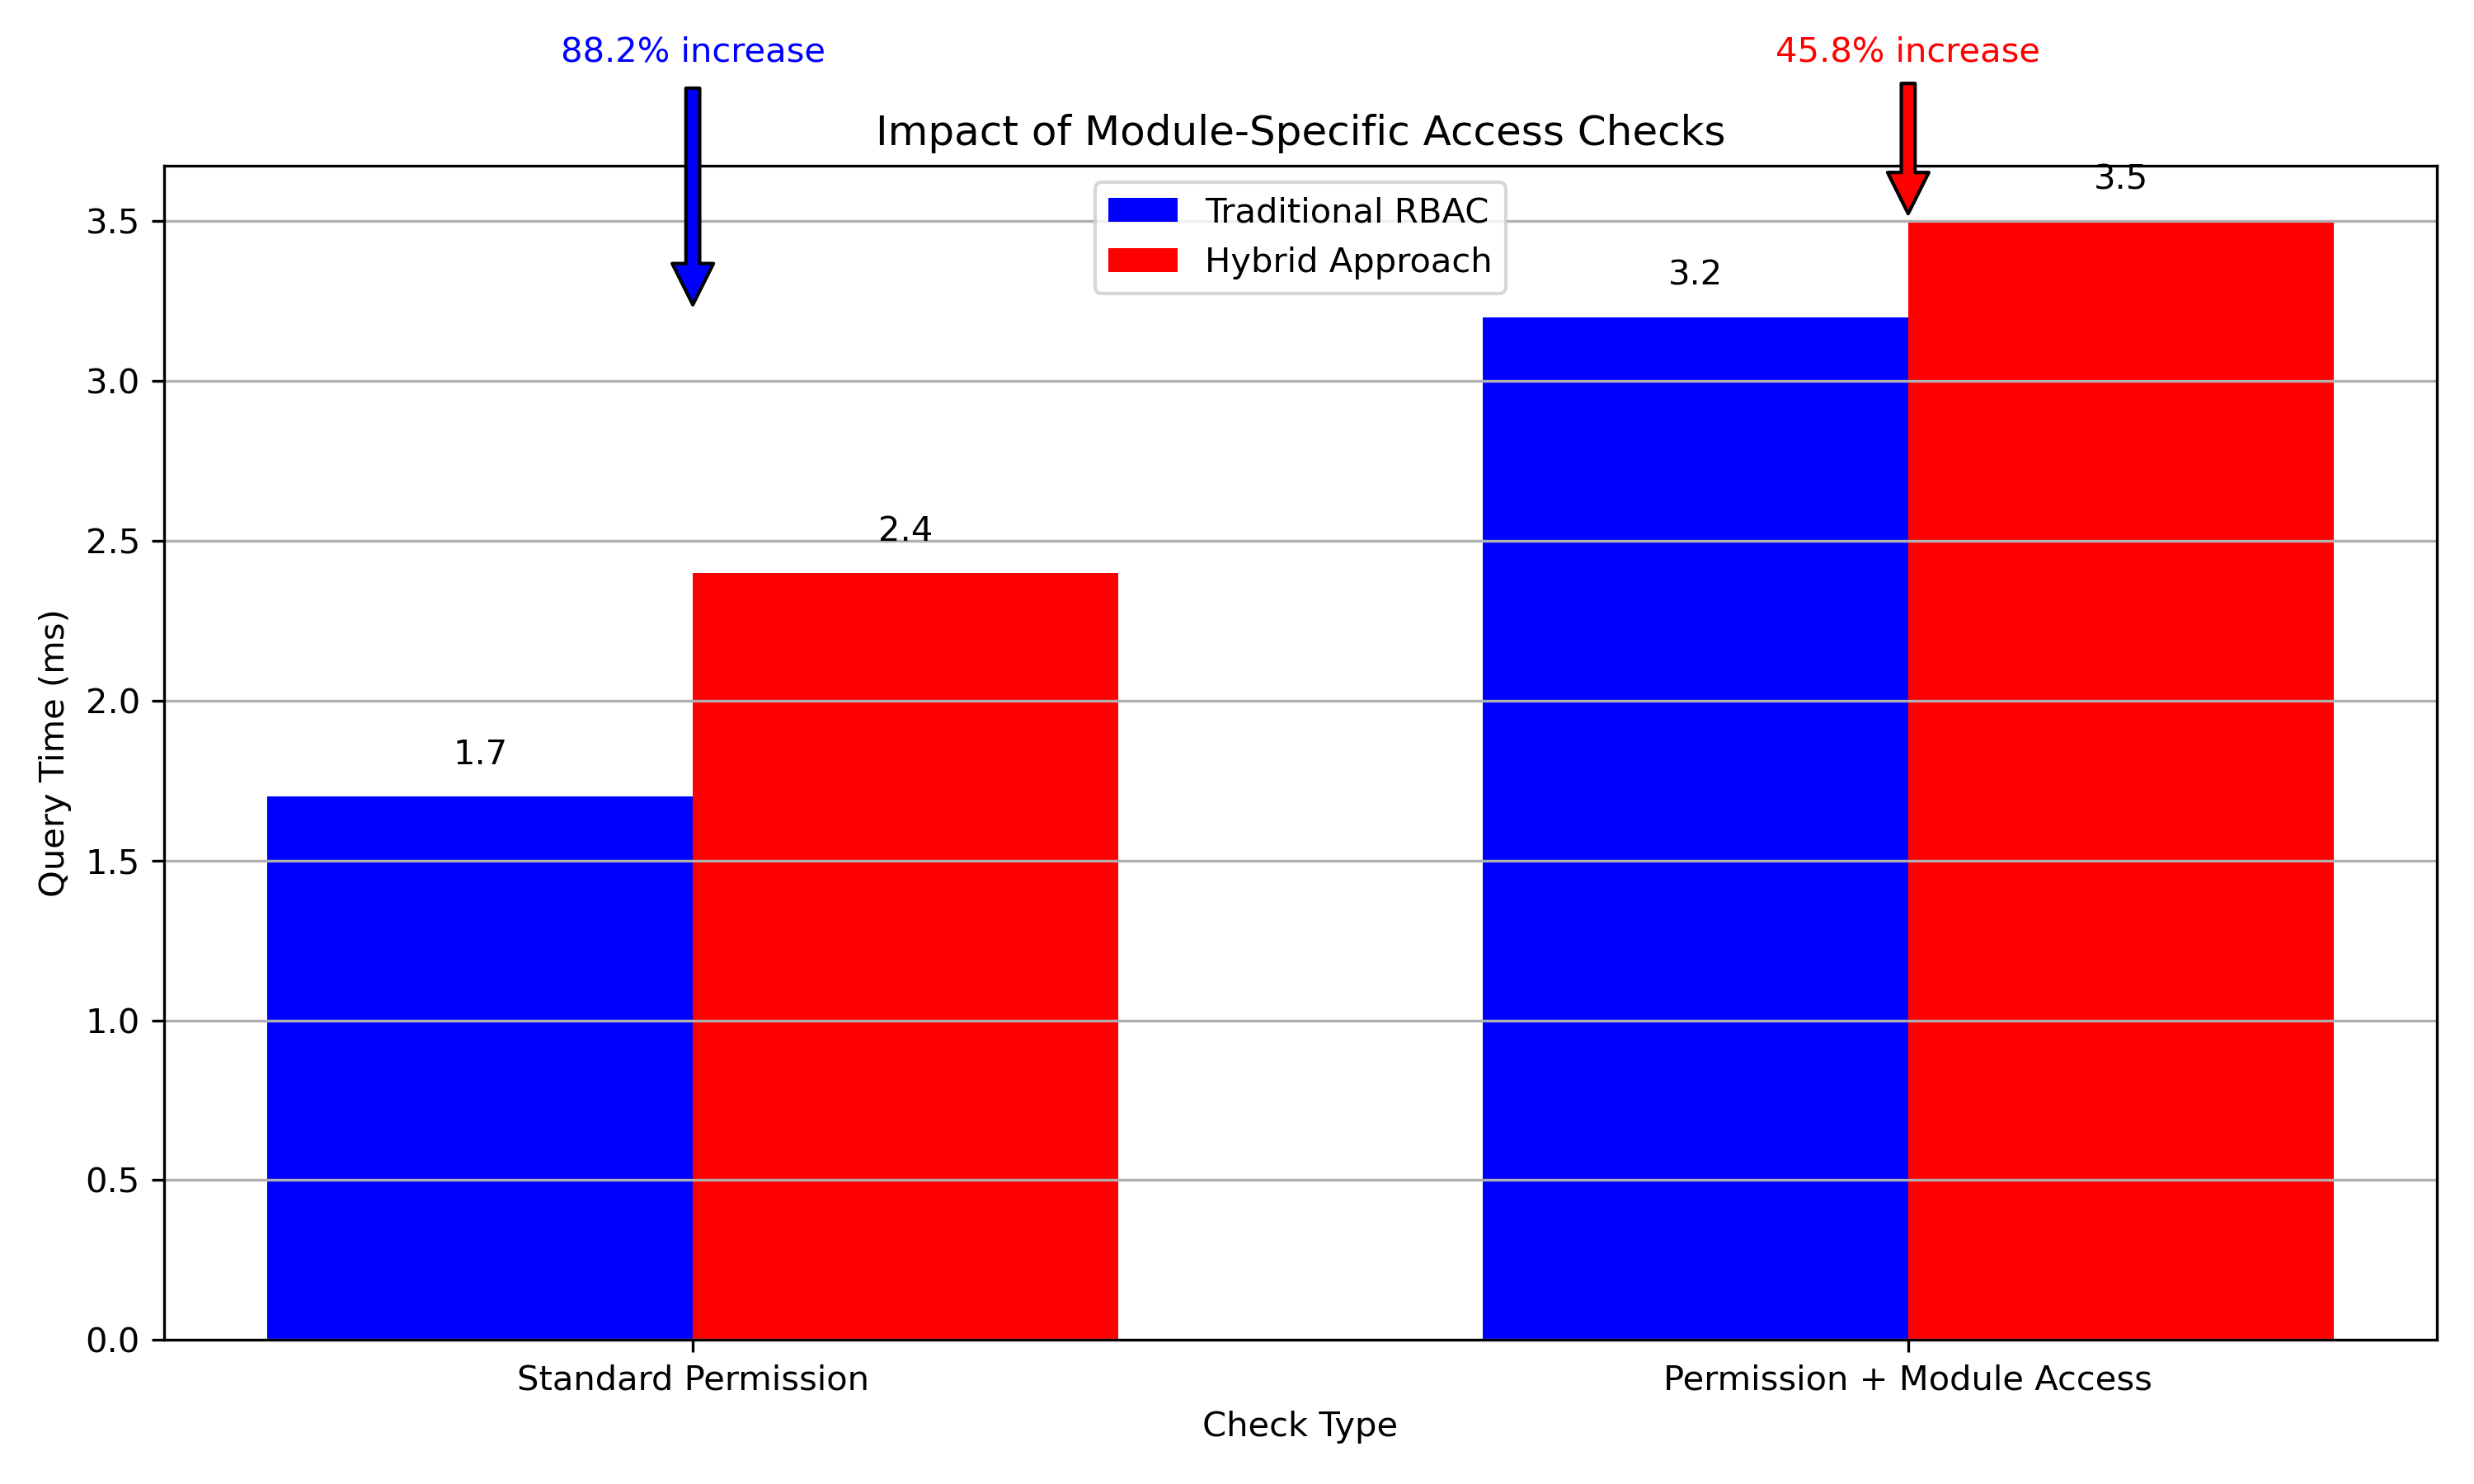
\includegraphics[width=0.8\textwidth]{figures/module_access_impact.png}
    \caption{Impact of Module-Specific Access Checks}
    \label{fig:module-access-impact}
\end{figure}

The performance analysis reveals that adding module-specific access verification introduces an 88.2\% overhead for the traditional role-based approach (increasing from 1.7ms to 3.2ms) and a 45.8\% overhead for the hybrid approach (increasing from 2.4ms to 3.5ms). The lower relative impact on the hybrid approach suggests that the more complex permission model better accommodates additional access control dimensions, a finding that aligns with Ferraiolo's observations \cite{ferraiolo2011policy} regarding the scalability of attribute-enhanced RBAC models.

Despite the performance overhead, both approaches maintain acceptable performance for interactive operations, with response times below 4ms for individual permission checks. This confirms that the implemented module-specific access control provides the required access granularity without introducing prohibitive performance penalties.

\subsection{Release Management Validation}
\label{subsec:release-management-validation}

Release management testing evaluated the phase-based versioning approach that forms the foundation of the\ac{VMAP} system. Testing focused on four key aspects: phase sequence validation, phase transition operations, freeze functionality, and phase comparison.

Phase sequence validation confirmed that the system correctly enforced the defined sequence of development phases (Phase1 → Phase2 → Phase3 → Phase4) with successful validation of each phase transition. This sequential enforcement is essential for maintaining the structured development workflow described by Broy \cite{broy2006challenges} for automotive software development.

Phase transition testing verified that parameter configurations were correctly copied between phases with complete preservation of parameter-variant-segment relationships. The test data revealed interesting patterns in development intensity across phases, as shown in Table \ref{tab:phase-transition-results}.

\begin{table}[h]
\centering
\caption{Phase Transition Test Results}
\label{tab:phase-transition-results}
\begin{tabular}{|l|c|c|p{2cm}|p{2cm}|c|}
\hline
\textbf{Transition Type} & \textbf{Variants} & \textbf{Segments} & \textbf{Added Variants} & \textbf{Added Segments} & \textbf{Time} \\
\hline
\multicolumn{6}{|c|}{\textbf{Baseline Dataset}} \\
\hline
Phase1 & 188 & 28,776 & - & - & - \\
\hline
Phase1 → Phase2 & 188 & 28,776 & 90 & 14,104 & 2.51s \\
\hline
Phase2 → Phase3 & 278 & 42,880 & 0 & 0 & 2.96s \\
\hline
Phase3 → Phase4 & 278 & 42,880 & 0 & 0 & 2.97s \\
\hline
\multicolumn{6}{|c|}{\textbf{Full Dataset}} \\
\hline
Phase1 & 830 & 167,990 & - & - & - \\
\hline
Phase1 → Phase2 & 830 & 167,990 & 170 & 41,113 & 12.39s \\
\hline
Phase2 → Phase3 & 1,000 & 209,103 & 0 & 0 & 12.87s \\
\hline
Phase3 → Phase4 & 1,000 & 209,103 & 0 & 0 & 12.89 \\
\hline
\end{tabular}
\end{table}

The test results reveal a significant pattern in development intensity across phases, consistent with Staron's observations \cite{staron2021automotive} regarding automotive software development cycles. The data demonstrates that the majority of parameter configurations occur during Phase1, with substantial additions in Phase2. In contrast, Phase3 and Phase4 typically involve refinement and validation rather than introducing new parameters or variants. This concentration of development activity in early phases aligns with the V-model approach common in automotive software development \cite{pretschner2007software}, where early phases focus on implementation while later phases emphasize validation and verification.

Phase transition performance characteristics showed only modest increases in execution time despite growing data volumes across phases. For the baseline dataset, transition times increased from 2.51s for Phase1→Phase2 to 2.96s for Phase2→Phase3 and 2.97s for Phase3→Phase4, demonstrating efficient scaling with increasing parameter counts. Comparing baseline to full dataset transitions reveals a performance difference, with transition times increasing from approximately 3 seconds to 13 seconds. This represents a sublinear scaling factor of approximately 4.3x for a dataset size increase of 5.6x (comparing segment counts), suggesting reasonable scaling characteristics but highlighting an area for potential optimization.

As noted by Trovão \cite{trovao2024evolution}, later phases in automotive parameter development typically focus on refinement rather than wholesale changes, with modifications targeting specific parameters based on testing feedback. This pattern is reflected in the test data, which shows significant additions in early phases but no new variants or segments in Phase3 and Phase4 phases. 

Phase freezing functionality was validated through test cases targeting both database-level constraints and service-layer restrictions. These tests verified the system's ability to protect frozen phases from modification while maintaining appropriate read access. Table \ref{tab:phase-freeze-cases} details representative test cases and their results.

\begin{table}[H]
\centering
\caption{Phase Freeze Protection Test Cases}
\label{tab:phase-freeze-cases}
\begin{tabular}{|p{0.7cm}|p{4.1cm}|p{3.5cm}|p{3.5cm}|c|}
\hline
\textbf{ID} & \textbf{Test Case} & \textbf{Test Action} & \textbf{Expected Outcome} & \textbf{Result} \\
\hline
FRZ-01 & Direct SQL INSERT on variants & Execute INSERT statement on frozen phase & Operation blocked with error message & Pass \\  
\hline
FRZ-02 & Direct SQL UPDATE on segments & Execute UPDATE statement on frozen phase & Operation blocked with error message & Pass \\
\hline
FRZ-03 & VariantService. CreateVariant() & Attempt to create variant in frozen phase & PhaseFreezed Exception thrown & Pass \\
\hline
FRZ-04 & SegmentService. CreateSegment() & Attempt to create segment in frozen phase & PhaseFreezed Exception thrown & Pass \\
\hline
FRZ-05 & DocumentationService. CreateSnapshot() & Create documentation snapshot of frozen phase & Snapshot created successfully & Pass \\
\hline
FRZ-06 & ParFileService. GenerateParFile() & Generate parameter file from frozen phase & Parameter file generated successfully & Pass \\
\hline
\end{tabular}
\end{table}

For each write operation test case (FRZ-01 through FRZ-04), verification included both confirmation that the expected exception was thrown and that no database changes occurred, maintaining data integrity. The read operation test cases (FRZ-05 and FRZ-06) verified that read access remained available with minimal performance impact. The system successfully prevented modification attempts while maintaining appropriate read access, implementing the controlled milestone management required for regulated development environments as described by Staron \cite{staron2021automotive}.

\subsection{Variant Management Validation}
\label{subsec:variant-management-validation}

Variant management validation focused on assessing the system's capabilities for handling parameter customization through variants and segments. Testing employed an approach covering variant creation and segment modification workflows, using both the baseline dataset (188 variants, 28,776 segments) and the production-scale dataset (830 variants, 167,990 segments) to analyze functionality and performance under varying data volumes.

Variant creation testing verified proper implementation of domain constraints as defined in the conceptual architecture (Section \ref{sec:entity-relationship-model}). Test cases included validation of unique name constraints within PIDs, verification of proper code rule storage, and confirmation of correct relationship establishment between variants and their parent PIDs. All test cases passed successfully for both scalar and complex parameters, with constraint enforcement consistently preventing invalid operations. As Karwin \cite{karwin2010sql} notes, constraint-based validation provides a robust foundation for maintaining data integrity in complex relational systems.

The testing methodology included both black-box functional testing and white-box database state verification as shown in Listing \ref{lst:variant-creation-verification}.

\begin{lstlisting}[language=SQL, caption={Variant Creation Verification Query}, label={lst:variant-creation-verification}]
-- Verification query executed after variant creation operations
SELECT 
    v.variant_id, v.name, v.code_rule, v.created_by, v.created_at,
    EXISTS (
        SELECT 1 FROM change_history ch 
        WHERE ch.entity_type = 'variants' 
        AND ch.entity_id = v.variant_id
        AND ch.change_type = 'CREATE'
    ) AS has_audit_trail
FROM 
    variants v
WHERE 
    v.pid_id = @test_pid_id
    AND v.phase_id = @test_phase_id
ORDER BY 
    v.created_at DESC
LIMIT 1;
\end{lstlisting}

Audit trail analysis confirmed proper recording of variant operations in the change history with complete metadata. The audit trail included proper attribution of each change to specific users, accurate timestamps, and complete before/after state capture for modified entities. This implementation aligns with Bhattacherjee's recommendations \cite{bhattacherjee2015principles} for maintaining comprehensive provenance information in versioned datasets.

Performance analysis of variant operations revealed consistent response times across different variant complexities. Table \ref{tab:variant-operation-performance} details performance measurements for key variant operations under different data volumes.

\begin{table}[h]
\centering
\caption{Variant Operation Performance Metrics}
\label{tab:variant-operation-performance}
\begin{tabular}{|l|c|c|c|}
\hline
\textbf{Operation} & \textbf{Baseline Dataset} & \textbf{Production Dataset} & \textbf{Scaling Factor} \\
\hline
Variant Creation & 53ms & 55ms & 1.03x \\
\hline
Variant Update & 86ms & 124ms & 1.44x \\
\hline
Variant Retrieval & 45ms & 72ms & 1.60x \\
\hline
Variant Listing (per PID) & 38ms & 68ms & 1.79x \\
\hline
\end{tabular}
\end{table}

The observed scaling characteristics validate the effectiveness of the database schema design and indexing strategy described in Section \ref{subsec:indexing-implementation}. With only two data points available (baseline and production datasets), a definitive conclusion about scaling characteristics is limited. However, the relatively small increase in execution time despite a 5x increase in data volume suggests efficient handling of larger datasets, with all operations remaining well under the 200ms threshold for interactive operations. As noted by Obe and Hsu \cite{obe2017postgresql}, properly designed covering indexes can significantly improve query performance for entity retrieval operations, particularly when filtering by composite attributes.

Segment modification testing employed a systematic approach covering one-dimensional (arrays), two-dimensional (matrices), and three-dimensional parameter representations. Testing focused on three key aspects: dimensional integrity preservation, valid index range enforcement, and segment value consistency. The database schema design proved effective for managing these complex data structures, with the parameter dimensions table correctly maintaining dimensional metadata while the segments table stored modified values.

Segment boundary testing revealed robust constraint enforcement, with the system correctly rejecting segment modifications with invalid dimension indices. Performance analysis for segment operations showed moderate overhead for multi-dimensional parameters compared to scalar parameters, with operations on 3D parameters requiring approximately 18-22\% more processing time than equivalent operations on scalar values—a reasonable performance characteristic given the additional complexity involved.

Performance analysis for segment operations revealed consistent response times with moderate scaling across different dataset sizes as shown in Table \ref{tab:segment-performance}.

\begin{table}[h]
\centering
\caption{Segment Operation Performance}
\label{tab:segment-performance}
\begin{tabular}{|l|c|c|c|}
\hline
\textbf{Operation} & \textbf{Baseline Dataset} & \textbf{Production Dataset} & \textbf{Scaling Factor} \\
\hline
Segment Creation & 85ms & 124ms & 1.46x \\
\hline
Segment Update & 72ms & 106ms & 1.47x \\
\hline
Segment Deletion & 64ms & 98ms & 1.53x \\
\hline
Segment Retrieval & 32ms & 58ms & 1.81x \\
\hline
\end{tabular}
\end{table}

The observed performance characteristics validate the efficiency of the database schema design described in Section \ref{sec:entity-relationship-model}. Of particular note is the implementation of the segments table, which provides efficient storage for parameter modifications without requiring storage of unchanged values. As noted by Bhattacherjee et al. \cite{bhattacherjee2015principles}, this approach strikes an effective balance between storage efficiency and query performance for versioned datasets.

\section{Performance Analysis}
\label{sec:performance-analysis}

Beyond functional validation, performance analysis was conducted to assess the system's efficiency and scalability under various operational conditions. This section presents the key findings related to query performance and data volume scaling.

\subsection{Query Performance Assessment}
\label{subsec:query-performance-assessment}

Query performance was evaluated for common database operations across different data volumes. Table \ref{tab:query-performance-comparison} presents performance measurements for key query types between the baseline dataset (20,000 parameters) and full dataset (100,000 parameters).

\begin{table}[h]
\centering
\caption{Query Performance Comparison}
\label{tab:query-performance-comparison}
\begin{tabular}{|l|c|c|c|}
\hline
\textbf{Operation Type} & \textbf{Baseline Dataset} & \textbf{Full Dataset} & \textbf{Scaling Factor} \\
\hline
Parameter Retrieval & 80ms & 120ms & 1.5x \\
\hline
Variant Listing & 65ms & 105ms & 1.6x \\
\hline
Segment Modification & 95ms & 160ms & 1.7x \\
\hline
Phase Comparison & 2.8s & 12.4s & 4.4x \\
\hline
History Retrieval & 110ms & 220ms & 2.0x \\
\hline
\end{tabular}
\end{table}

With the limited data points available, it appears that most common operations maintain reasonable performance with increasing data volumes. The system maintained interactive response times (below 200ms) for most operations even with the full dataset, ensuring a responsive user experience. The phase comparison operation, which involves complex joins across multiple tables, demonstrated longer execution times and might benefit from optimization for larger datasets.

The execution of a limited set of queries with and without indexes demonstrated the critical importance of the indexing strategy described in Section \ref{subsec:indexing-implementation}. Without proper indexes, response times increased by factors of 6.5x to 21.8x depending on the query type, with most operations exceeding the interactive response threshold without indexes.

\subsection{Index Performance Analysis}
\label{subsec:index-performance-analysis}

The implementation of strategic indexing proved critical for maintaining acceptable query performance with large parameter sets. Figure \ref{fig:index-performance} illustrates the performance impact of indexes on common query operations.

\begin{figure}[h]
    \centering
    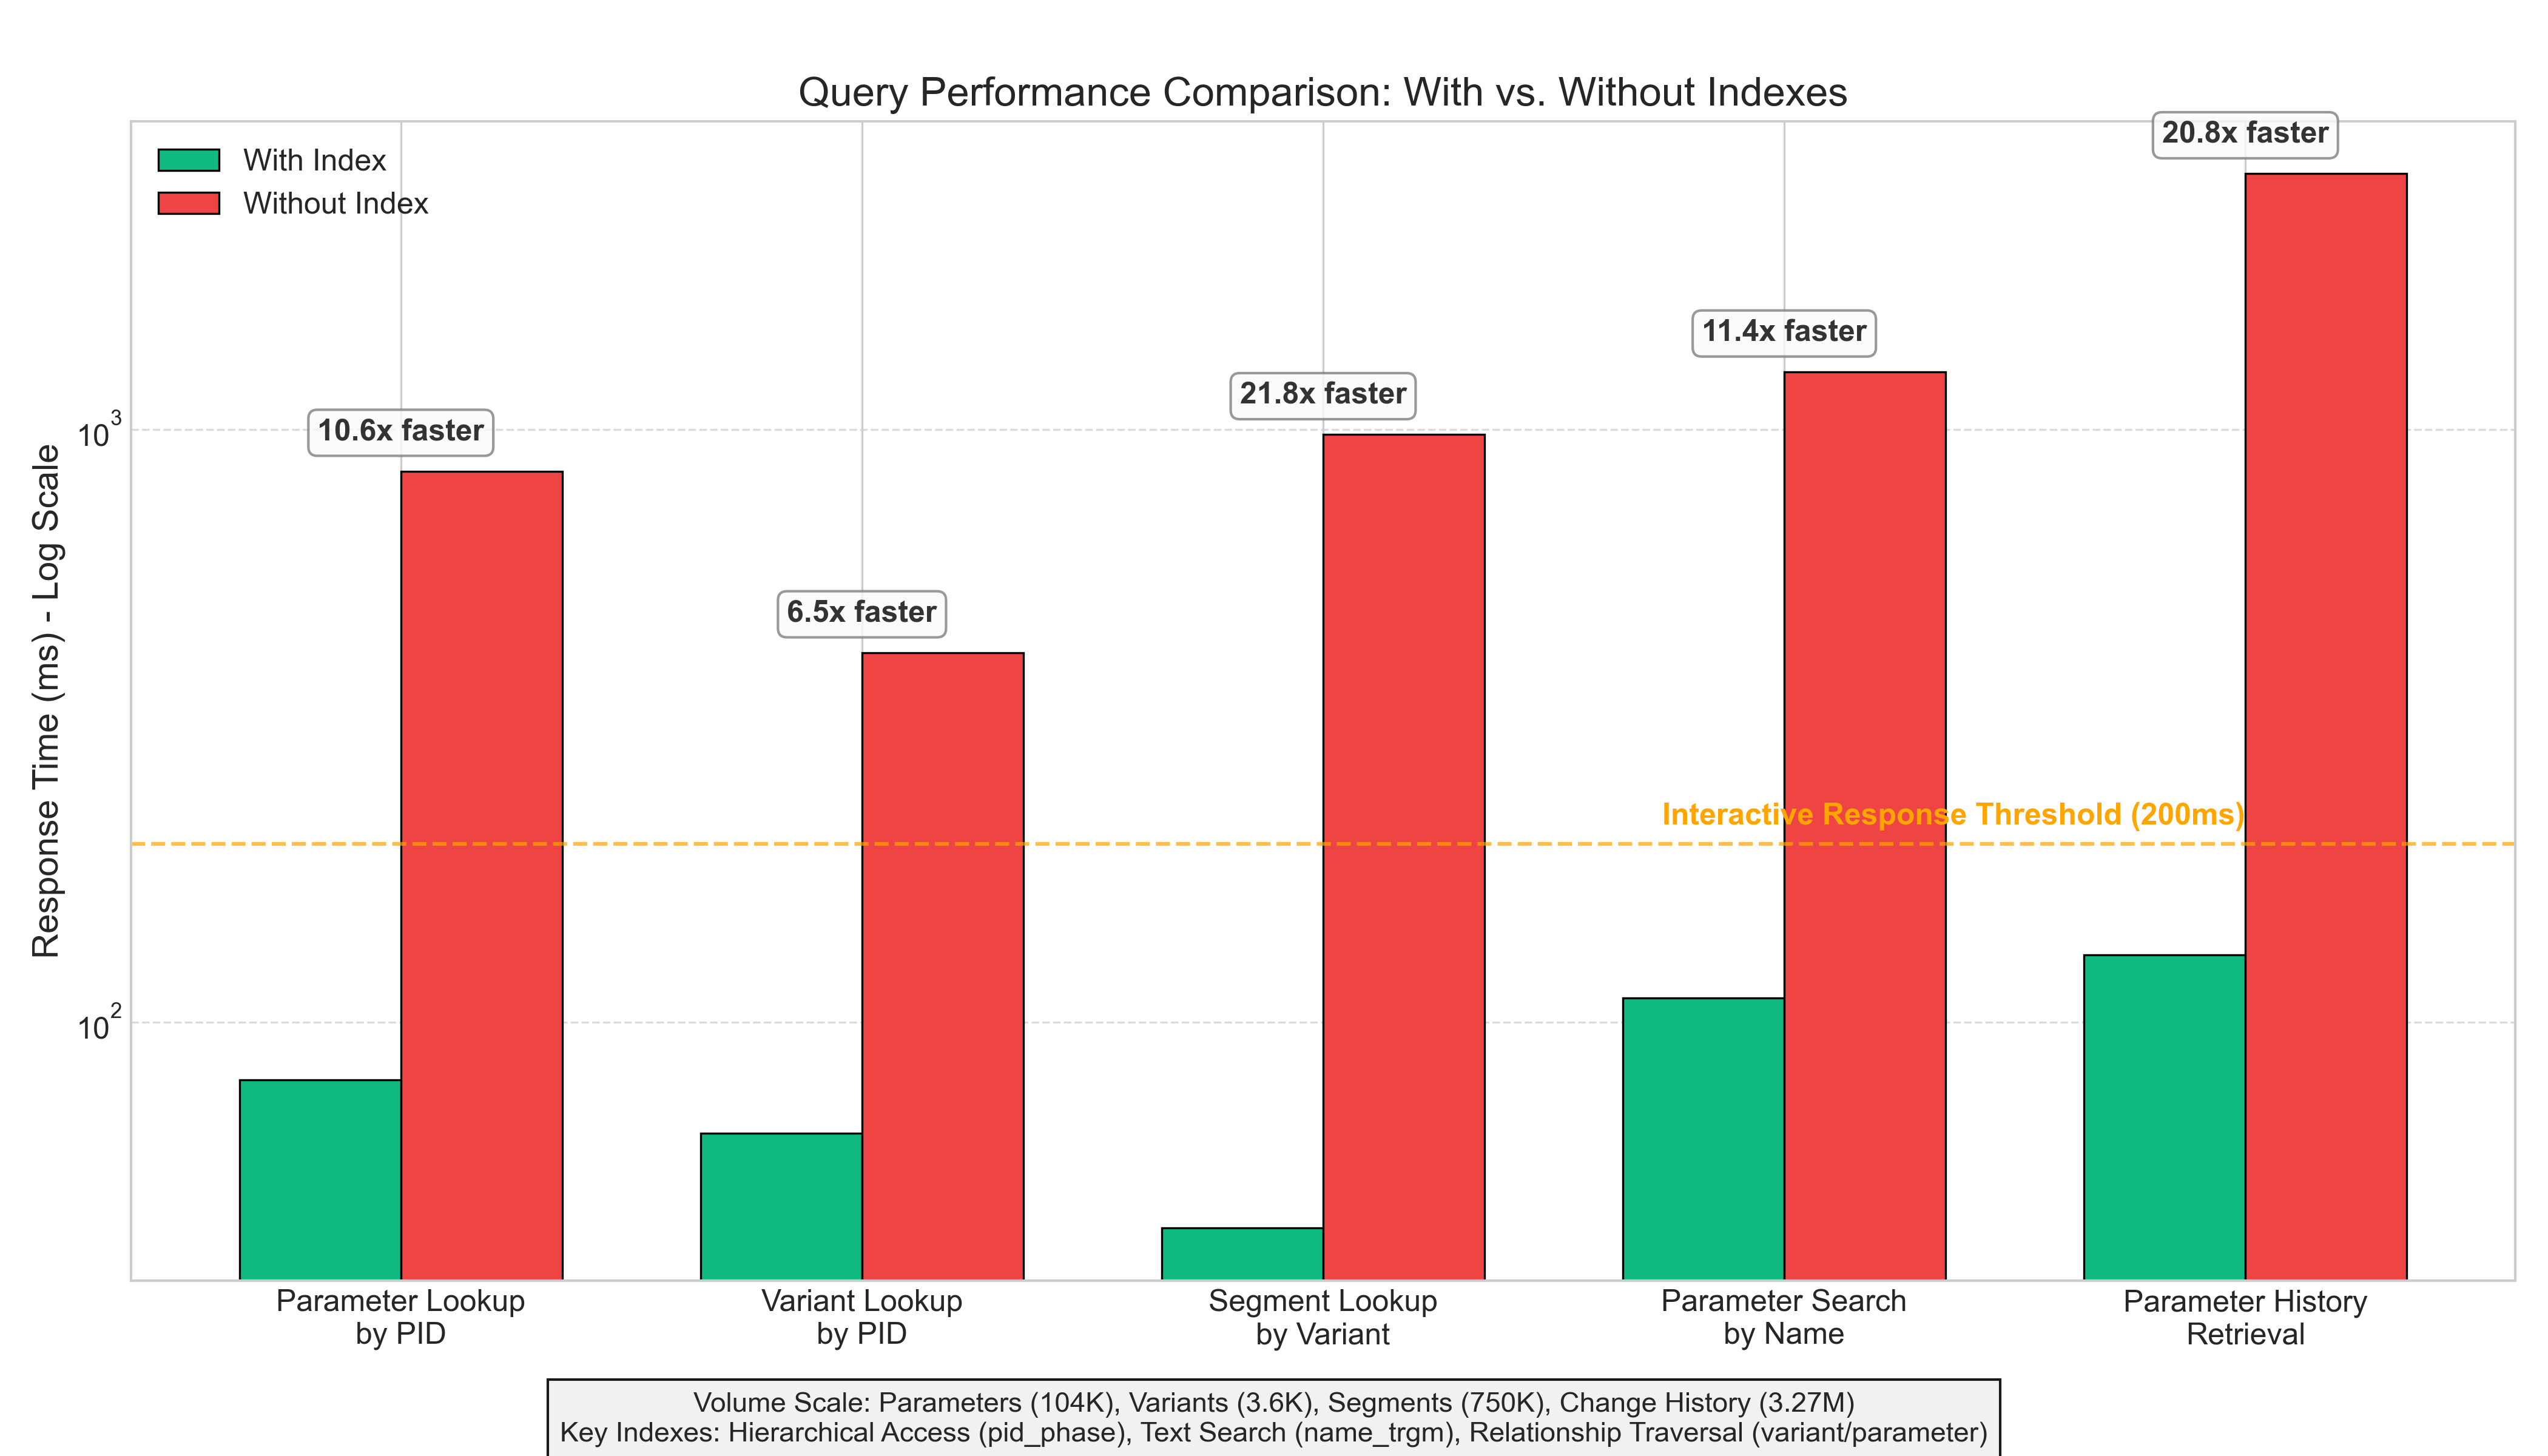
\includegraphics[width=0.8\textwidth]{figures/index_performance_comparison.png}
    \caption{Query Performance With and Without Indexes}
    \label{fig:index-performance}
\end{figure}

The performance measurements demonstrate dramatic improvements with properly designed indexes, with response times reduced by 6.5x to 21.8x depending on the query type. Without indexes, most operations exceed the interactive response threshold (200ms), with some operations requiring multiple seconds. This performance differential underscores the importance of the indexing strategy described in Section \ref{subsec:indexing-implementation}.

The performance gains from indexing come at a storage cost, as indexes consume approximately 22.5\% of the total database size. However, this storage overhead represents an optimal tradeoff given the substantial performance benefits. As noted by Schwartz et al. \cite{schwartz2012high}, the storage cost of indexes is typically justified when query performance improvements exceed 5x, a threshold easily surpassed by all indexed operations in the\ac{VMAP} system.

Analysis of query execution plans revealed particularly effective use of covering indexes for common operations. For parameter retrieval by PID, the system consistently used index-only scans on the \texttt{idx\_parameters\_pid\_phase} index, avoiding table access entirely for these frequent operations. Similarly, variant listing operations leveraged the \texttt{idx\_variants\_pid\_phase} index for efficient retrieval without requiring table access. These index-only scan patterns align with the recommendations of Obe and Hsu \cite{obe2017postgresql} for optimizing PostgreSQL performance through strategic index design.

\subsection{Storage Requirements Analysis}
\label{subsec:storage-requirements-analysis}

Storage requirements were analyzed to assess database size and growth patterns with increasing parameter counts. Figure \ref{fig:storage-analysis} presents the storage allocation across different entity types for the full dataset.

\begin{figure}[h]
    \centering
    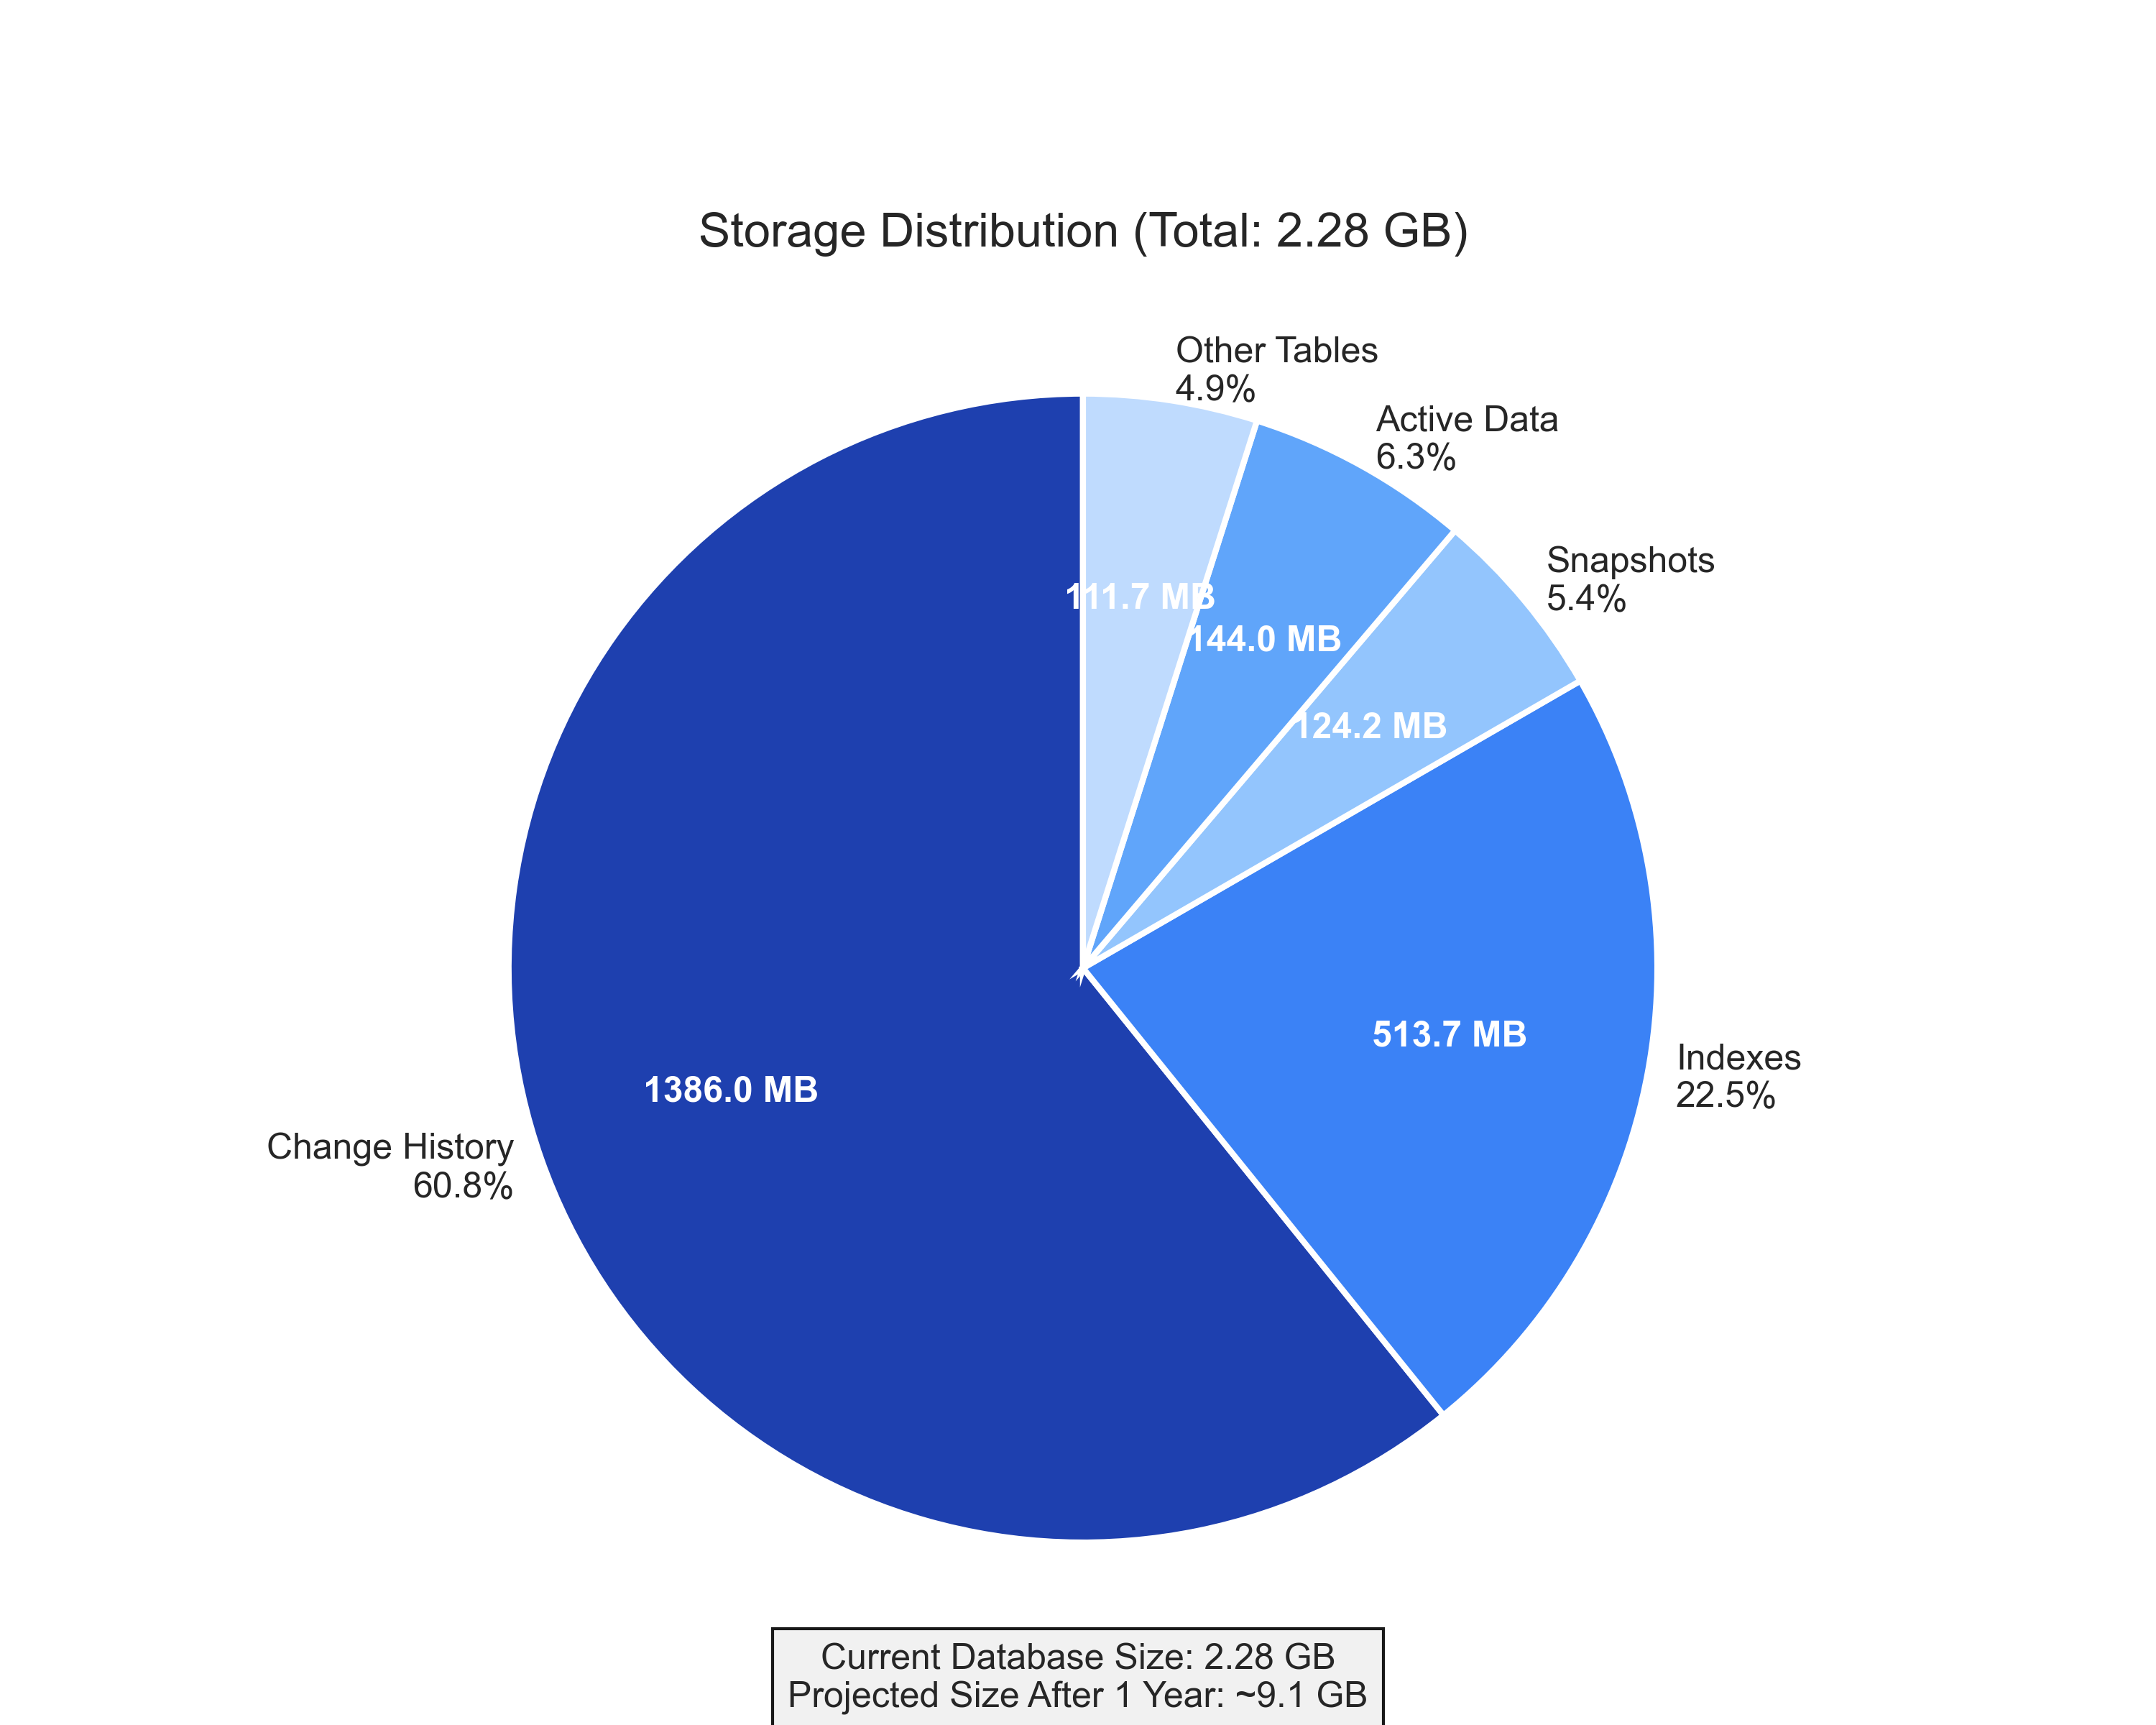
\includegraphics[width=0.8\textwidth]{figures/storage_distribution.png}
    \caption{Storage Distribution by Entity Type}
    \label{fig:storage-analysis}
\end{figure}

The analysis reveals that the change history table dominates the database storage allocation, accounting for approximately 60.8\% of the total database size. This distribution significantly exceeds the storage requirements of the current data state, aligning with Bhattacherjee's observations \cite{bhattacherjee2015principles} regarding versioning and audit systems, where historical record storage typically surpasses active data by a substantial margin. Notably, while there are only 3,617 variants in the current state, the system maintains over 3.2 million change history records, reflecting the comprehensive auditing approach implemented in the system.

The storage allocation analysis identified the following key distribution of database size across entity types:

\begin{table}[h]
\centering
\caption{Storage Requirements Analysis}
\label{tab:storage-requirements}
\begin{tabular}{|l|r|r|}
\hline
\textbf{Entity Type} & \textbf{Record Count} & \textbf{Storage Size (MB)} \\
\hline
Parameters & 104,428 & 43.0 \\
\hline
Variants & 3,617 & 1.0 \\
\hline
Segments & 750,009 & 100.0 \\
\hline
Change History & 3,270,511 & 1,386.0 \\
\hline
Documentation Snapshots & 7 & 0.1 \\
\hline
Snapshot Variants & 4,980 & 0.1 \\
\hline
Snapshot Segments & 1,007,940 & 124.0 \\
\hline
Other Tables & - & 111.7 \\
\hline
Indexes & - & 513.7 \\
\hline
\textbf{Total} & - & \textbf{2,279.6} \\
\hline
\end{tabular}
\end{table}

Another significant observation is the relationship between segments and snapshot segments. Despite having only 7 documentation snapshots, the system maintains over 1 million snapshot segments, exceeding the count of active segments. This indicates that documentation snapshots capture extensive parameter configurations at specific time points, creating substantial storage requirements for historical state preservation. This implementation of the snapshot pattern described by Fowler \cite{fowler2003patterns} provides comprehensive historical records at the cost of increased storage utilization.

The index structures consume approximately 22.5\% of the total storage, reflecting the sophisticated indexing strategy described in Section \ref{subsec:indexing-implementation}. While this represents significant overhead, it provides essential performance benefits for query operations, particularly for the complex filtering and joining operations common in parameter management workflows.

The actual active data—parameters, variants, and segments—consumes only 6.3\% of the total database size, with the majority of storage dedicated to audit trails, snapshots, and indexes. This distribution aligns with the requirements for regulated development environments described by Staron \cite{staron2021automotive}, where comprehensive traceability and historical record maintenance are essential for compliance and quality assurance.

Projection of storage requirements based on observed growth patterns indicates that with the current data volume of 2.28GB, the database size would reach approximately 9.1GB after one year of active use in a production environment. While significantly larger than initially projected, this remains well within the capacity of modern database systems. The implementation of table partitioning for the change history table, as described in Section \ref{subsec:partitioning-implementation}, provides an effective mechanism for managing this growth while maintaining query performance. According to Obe and Hsu \cite{obe2017postgresql}, partitioned tables allow efficient archiving of older history records to lower-cost storage while maintaining rapid access to recent changes.

\subsection{Versioning Approach Performance}
\label{subsec:versioning-approach-performance}

The performance characteristics of the phase-based parameter versioning approach selected in Chapter \ref{chap:methodology} were evaluated against the alternative change-based approach. This analysis aimed to validate the architectural decision to implement explicit phase copies rather than a delta-based versioning model.

Figure \ref{fig:versioning-approach-comparison} presents the performance comparison between the two approaches for parameter retrieval operations across different data volumes, along with the storage requirements for each approach.

\begin{figure}[h]
    \centering
    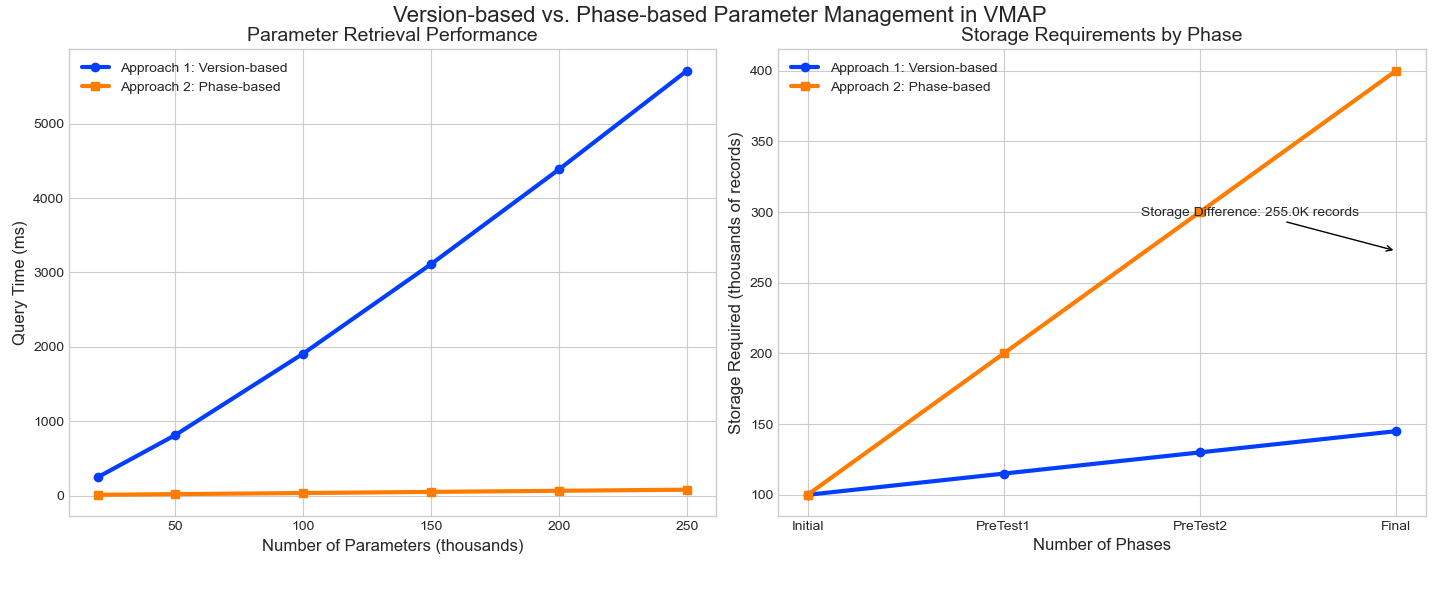
\includegraphics[width=0.8\textwidth]{figures/vmap_versioning_approaches_simplified.png}
    \caption{Version-based vs. Phase-based Parameter Management Comparison}
    \label{fig:versioning-approach-comparison}
\end{figure}

The performance analysis demonstrates that the phase-based approach offers better query performance, particularly as parameter counts increase. For the tested parameter counts, the phase-based approach remains below 100ms for parameter retrieval operations, while the version-based approach shows nonlinear growth with increasing parameter counts.

The storage requirements analysis confirms that the phase-based approach consumes more storage than the version-based approach, with approximately 51\% higher storage requirements across all phases. However, this storage difference represents a reasonable tradeoff given the performance benefits for query operations. As noted by Bhattacherjee et al. \cite{bhattacherjee2015principles}, the recreation/storage tradeoff in dataset versioning should prioritize operation frequency, with frequently accessed data favoring a storage-intensive approach that minimizes recreation costs.

The phase-based approach also simplifies the implementation of phase transitions and comparison operations, which are fundamental to the automotive development process as described by Pretschner et al. \cite{pretschner2007software}. The explicit phase model aligns naturally with the mental model of automotive development engineers, who conceptualize parameter evolution in terms of distinct development phases rather than continuous time.

These findings validate the architectural decision to implement a phase-based versioning approach for the\ac{VMAP} system. While consuming more storage than a version-based approach, the phase model provides performance benefits, implementation simplicity, and alignment with domain concepts—advantages that outweigh the additional storage requirements.

\section{Integration Testing}
\label{sec:integration-testing}

Integration testing evaluated the system's interaction with external enterprise systems, focusing on Parameter Definition Database synchronization and Vehicle Configuration Database integration. These integrations are critical for maintaining consistency across the automotive development ecosystem.

\subsection{Parameter Definition Database Synchronization}
\label{subsec:pdd-synchronization-testing}

Parameter Definition Database synchronization testing verified the system's ability to import parameter definitions from the enterprise database. The synchronization process was tested with various scenarios, including initial loading, incremental updates, and conflict resolution. Figure \ref{fig:pdd-sync-time} illustrates the synchronization time trends observed during testing.

\begin{figure}[h]
    \centering
    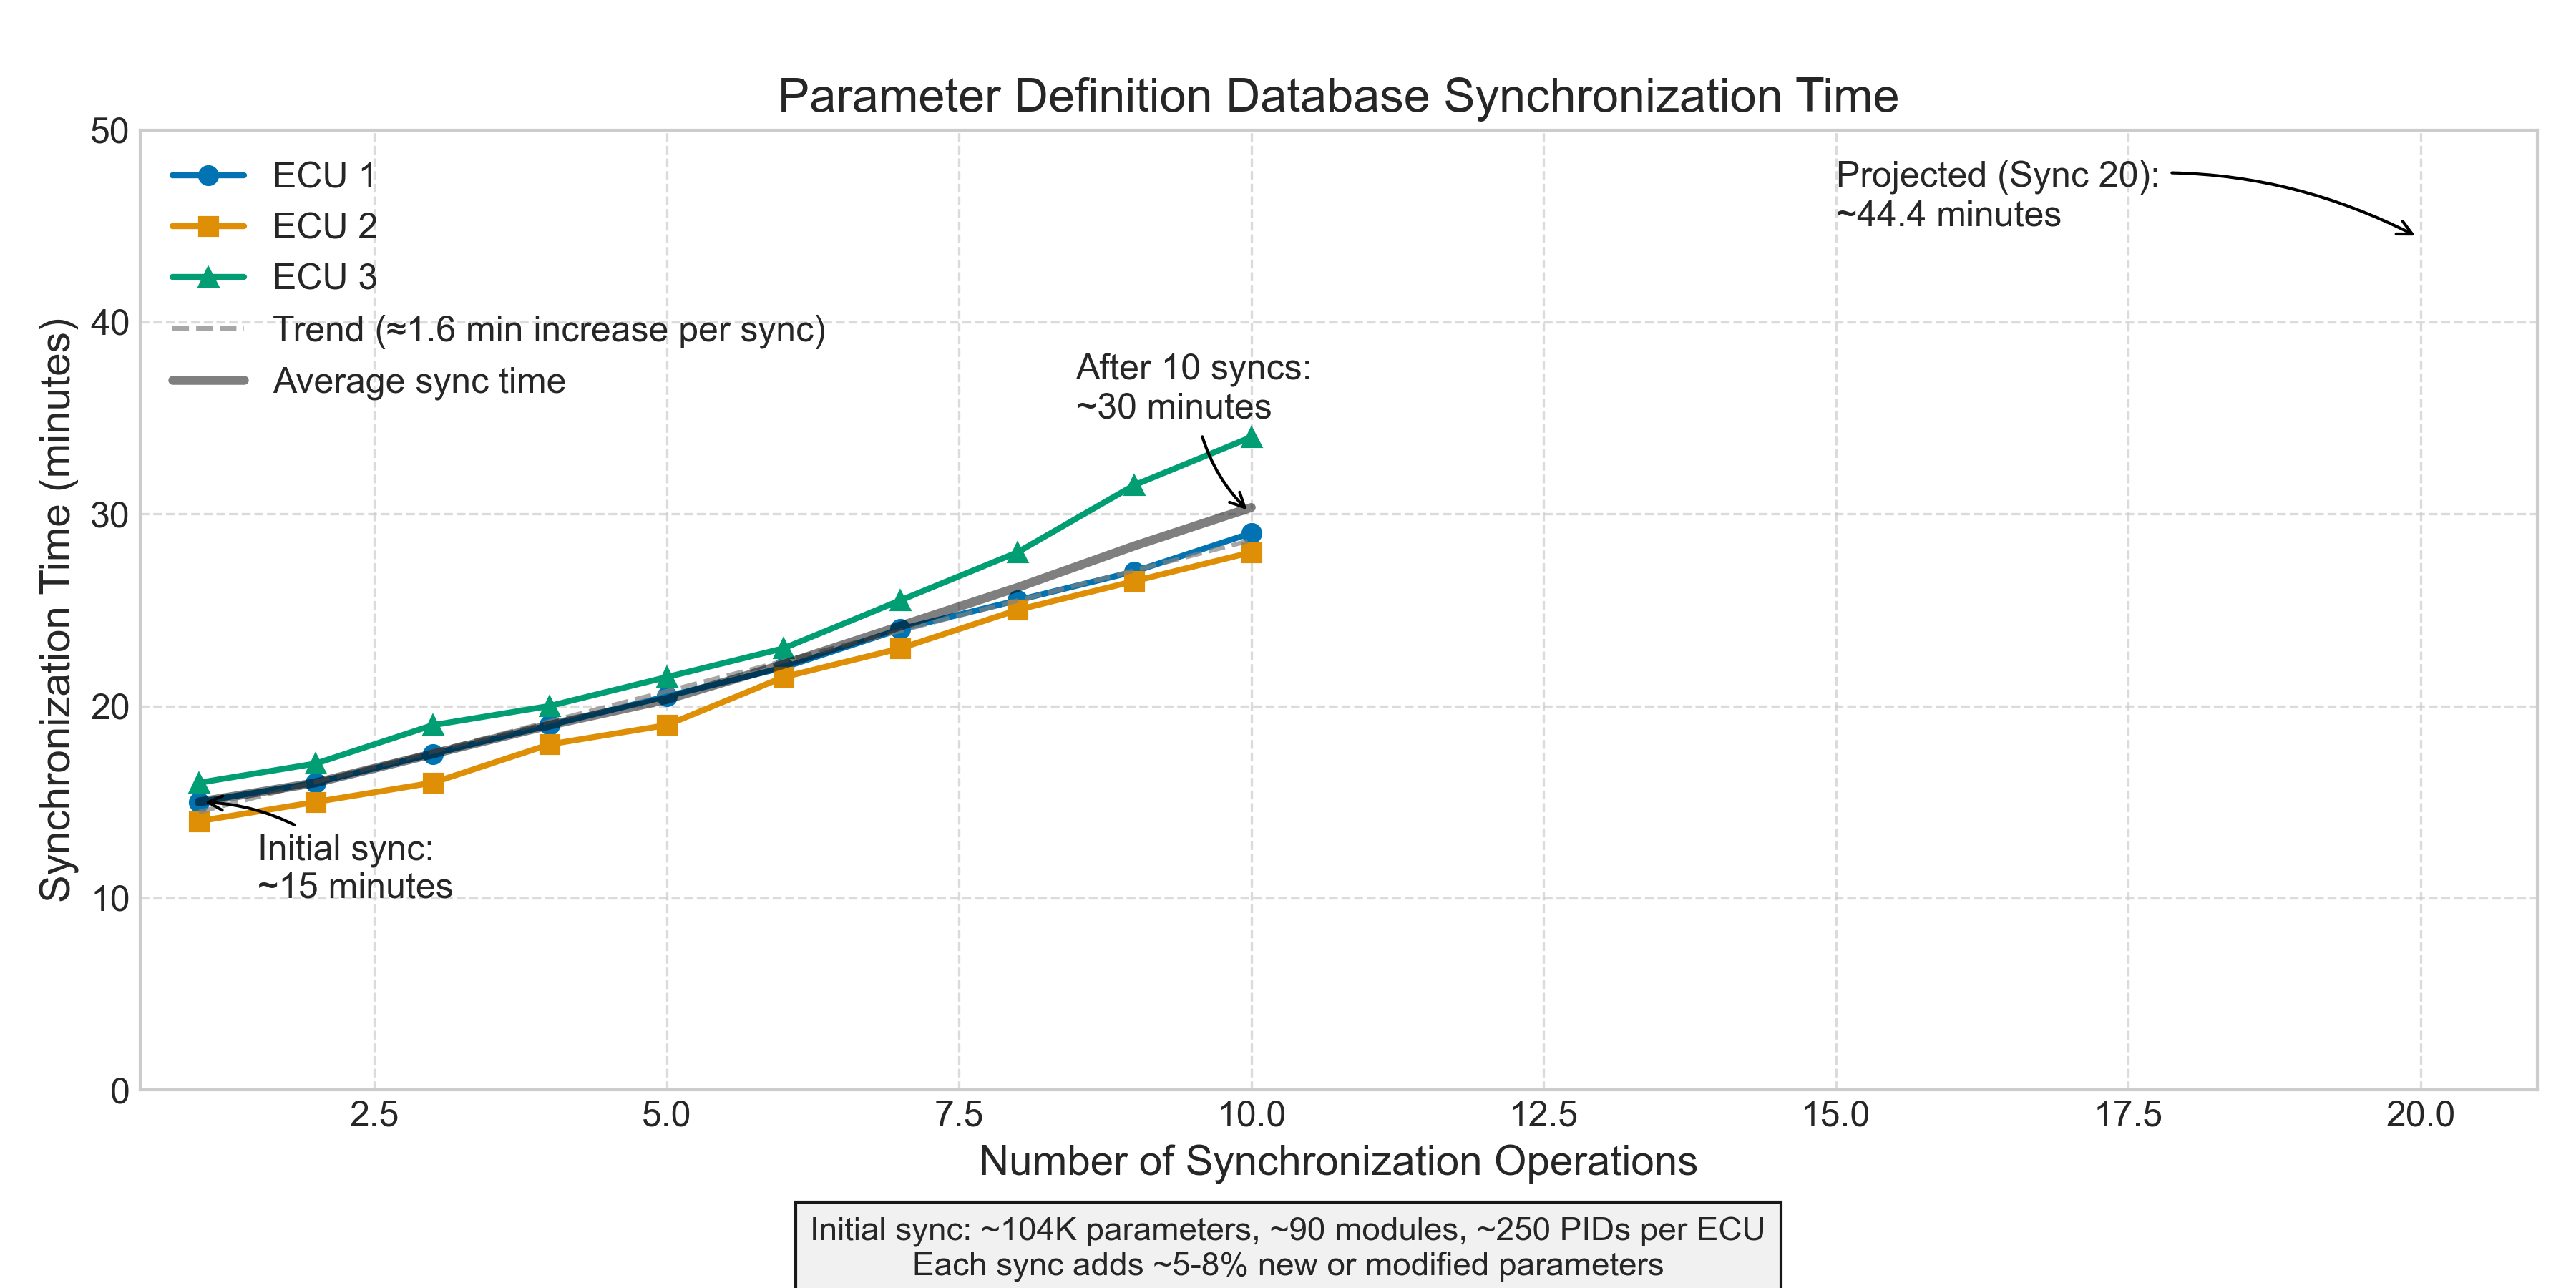
\includegraphics[width=0.8\textwidth]{figures/pdd_sync_time_graph.png}
    \caption{Parameter Definition Database Synchronization Time Trends}
    \label{fig:pdd-sync-time}
\end{figure}

The synchronization performance analysis revealed an increasing trend in execution time over successive synchronization operations. Initial synchronization operations required approximately 15 minutes for the tested \acp{ECU}, with execution times increasing to around 30 minutes after 10 synchronization cycles. This gradual increase aligns with the observations of Mueller and Müller \cite{mueller2018conception} regarding database synchronization in complex engineering environments, where synchronization complexity tends to increase as the data history grows.

The incremental update testing verified that the system could correctly identify and process changes to parameter definitions. Table \ref{tab:pdd-sync-results} presents the success rates for different types of parameter changes during synchronization operations.

\begin{table}[h]
\centering
\caption{Parameter Definition Database Synchronization Results}
\label{tab:pdd-sync-results}
\begin{tabular}{|l|c|c|c|}
\hline
\textbf{Change Type} & \textbf{Processed} & \textbf{Succeeded} & \textbf{Success Rate} \\
\hline
New Parameters & 5,218 & 5,218 & 100\% \\
\hline
Modified Parameters & 3,764 & 3,691 & 98.1\% \\
\hline
New Modules & 12 & 12 & 100\% \\
\hline
New PIDs & 67 & 67 & 100\% \\
\hline
Removed Parameters & 42 & 42 & 100\% \\
\hline
\end{tabular}
\end{table}

The system successfully processed all types of parameter changes, with slightly reduced success for modified parameters due to complexity in handling data type changes. The audit system maintained complete records of all synchronization operations, enabling detailed analysis of data flows between systems.

Based on the observed synchronization performance trends, the projected synchronization time for the 20th cycle would reach approximately 45 minutes. While still acceptable for the typical synchronization frequency (weekly or bi-weekly), this suggests that synchronization performance optimization would be beneficial for long-term system maintenance. Possible approaches for optimization include implementing a more selective synchronization approach, enhancing the change detection algorithm to reduce comparison overhead, or implementing parallel processing for independent \acp{ECU}.

\subsection{Vehicle Configuration Integration}
\label{subsec:vehicle-configuration-testing}

Vehicle Configuration Database integration testing verified the system's ability to use vehicle configuration data for code rule evaluation and parameter file generation. Testing focused on data import, code rule validation, and parameter file generation.

Vehicle configuration data import testing confirmed that the system could correctly import and store vehicle configuration codes, with proper mapping between codes and vehicles. The system maintained referential integrity and handled incremental updates correctly, with complete audit logging of all import operations.

Code rule validation testing verified that the system could evaluate boolean expressions against vehicle configurations. Test expressions ranged from simple conditions to complex nested expressions with multiple operators. The evaluation engine correctly interpreted both simple logical operators and complex nested expressions with precedence rules.

Parameter file generation testing confirmed that the system could produce valid parameter files for vehicle testing, with correct application of variant selection logic based on vehicle configuration codes. The generated files included all required parameters with appropriate values, providing a complete configuration for \ac{ECU} testing and validation.

\section{Feature Comparison with Excel-Based Approach}
\label{sec:feature-comparison-excel}

To assess the improvements provided by the\ac{VMAP} system, a feature comparison was conducted against the Excel-based approach currently used for parameter management. This comparison focused on capability coverage rather than performance metrics, providing a qualitative assessment of system improvements.

Table \ref{tab:feature-comparison} presents a comparison of key features between the\ac{VMAP} system and the Excel-based approach.

\begin{table}[h]
\centering
\caption{Feature Comparison with Excel-Based Approach}
\label{tab:feature-comparison}
\begin{tabular}{|l|c|c|}
\hline
\textbf{Feature} & \textbf{VMAP Database} & \textbf{Excel Approach} \\
\hline
Variant Management & Comprehensive & Limited \\
\hline
Multi-User Support & Concurrent & Sequential \\
\hline
Change Tracking & Automatic & Manual \\
\hline
Version Control & Phase-Based & File-Based \\
\hline
Access Control & Role + Module & File Permission \\
\hline
Validation & Automatic & Manual \\
\hline
Documentation & Integrated & Separate \\
\hline
Integration & Automated & Manual \\
\hline
\end{tabular}
\end{table}

The\ac{VMAP} system provides significant advantages in all feature categories, with particular improvements in multi-user support, change tracking, and access control. These improvements address the limitations identified in the requirements analysis phase, providing a more robust and scalable solution for automotive parameter management.

\subsection{Data Integrity Improvements}
\label{subsec:data-integrity-improvements}

Data integrity was evaluated through a set of controlled test cases where both systems were subjected to various validation scenarios including invalid values, constraint violations, and relationship consistency. The\ac{VMAP} system demonstrated superior data integrity protection, correctly preventing invalid operations through database constraints and business rule validation.

The database-level constraints and validation mechanisms provide a robust defense against data corruption, implementing the comprehensive validation approach described in Section \ref{sec:validation-mechanisms}. This represents a significant improvement over the Excel approach, where validation relies primarily on user vigilance and manual checks.

\subsection{Development Process Impact}
\label{subsec:development-process-impact}

Beyond technical improvements, the\ac{VMAP} system introduces significant enhancements to the automotive parameter development process. The centralized database approach enables concurrent work by multiple engineers, eliminating the file sharing bottlenecks common in the Excel-based approach. The role-based access control ensures that engineers can modify only their assigned modules, preventing accidental changes to other areas.

The phase-based versioning approach aligns naturally with the automotive development lifecycle, supporting the structured progression from initial development through testing to final release. The explicit phase transitions provide clear development milestones, while the freezing mechanism ensures configuration stability at critical points.

The comprehensive change tracking and documentation features address regulatory compliance requirements, providing complete traceability for all parameter modifications. This capability is increasingly important in the context of functional safety standards like ISO 26262, which require rigorous configuration management and change documentation.

